\documentclass{article}
\usepackage[utf8]{inputenc}
\usepackage{graphicx,wrapfig,lipsum}
\usepackage{subfigure}
\usepackage{geometry}
\usepackage{amsmath}
\newcommand{\euler}{e}
\newcommand{\ramuno}{i}
% proportions du docc
 \geometry{
 a4paper,
 total={170mm,257mm},
 left=20mm,
 top=20mm,
 }
 
 
\title{Projet : modélisation de pics de production de ressources }
\author{Yoan Thomas\and  Aya Ismahene Kroussa\and Melvin Cerba}

\begin{document}
% Page de garde
\begin{figure}
        \center
        
\includegraphics[scale = 0.4]{graphes/fig1.png}
\end{figure}
\maketitle
\begin{figure}[h]
        \center
        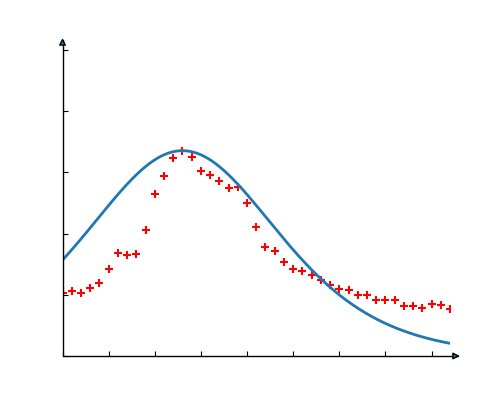
\includegraphics[scale = 1]{graphes/Courbe_de_Hubbert_Data.png}
\end{figure}


% Sommaire
\newpage
\vspace*{\fill}
\tableofcontents
\vspace*{\fill}


%
\newpage

\section{Élément historique}
% Explication des motivations du rapport %
$\indent$ Peut-on prédire l'évolution de la production des ressources non renouvelables ? Pour tenter de répondre à cette question, nous proposons d'étudier à travers ce projet certains outils mathématiques qui permettent de modéliser la production des ressources non renouvelables. Plus spécifiquement, nous nous intéresserons à la production de pétrole.



\subsection{Modélisation des pics de productions}
% Contexte historique et pratique %
\begin{wrapfigure}{r}{5.5cm}
	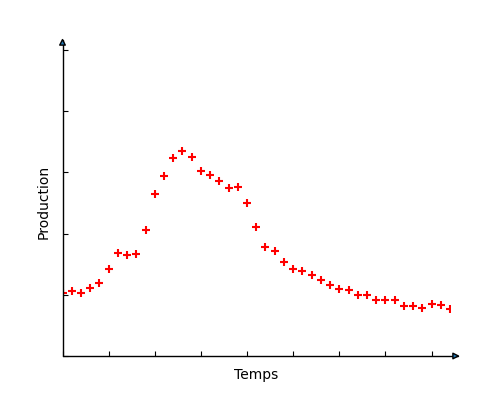
\includegraphics[width=5.5cm]{graphes/Production.png}
	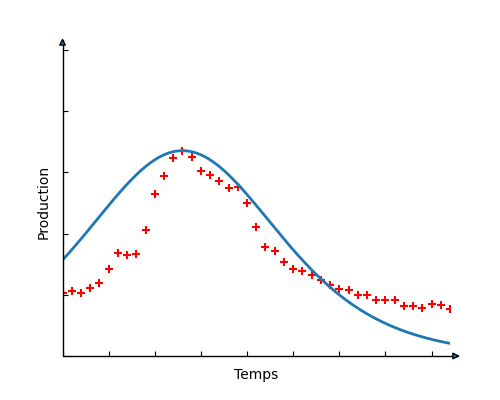
\includegraphics[width=5.5cm]{graphes/DataEtHubbert.png}
\end{wrapfigure} 
$\indent$ Être capable de prédire l'évolution de la production de diverses ressources a toujours été un enjeu majeur, notamment en économie. Il est donc naturel que de nombreux modèles mathématiques promettant de modéliser cette évolution soient apparus. A travers ce projet, nous vous proposons d'étudier en détail l'un d'eux : la courbe de Hubbert. \\
$\indent$ En 1956, Marion King Hubbert présentait sa "courbe de Hubbert" à l'American Petroleum Institute. Son modèle, qui postule que la production  croit, atteint un unique pic, puis décroit au même rythme qu'elle a augmenté en premier lieu, ne fit pas beaucoup parler de lui à l'époque. Mais lorsqu'en 1971, conformément à ses prédictions, la production pétrolière américaine atteignit son maximum et commença à décliner, ses travaux furent réexaminés avec beaucoup plus d'intérêt. Les chocs pétroliers de 1973 et 1979 semblèrent cependant définitivement invalider son modèle, qui perdit rapidement l'attention de l'industrie pétrolière.  \\
$\indent$ Malgré tout, l'avènement du calcul informatique et la grande disponibilité de données poussèrent des auteurs modernes à exhumer le modèle de Hubbert et à l'étendre, notamment en donnant une formule mathématique à sa courbe, permettant ainsi de calculer son intégrale. C'est sur la base de ces nouveaux travaux que nous avons construit notre projet.\\ \\



\subsection{Courbe de Hubbert et sigmoïde}
% Introduction du modèle mathématique et explication des paramètres %
$\indent$ Les auteurs qui se sont rapproprié la courbe de Hubbert ont notamment travaillé à lui donner une expression mathématique. Ceci leur a permis de définir son intégrale, que nous appellerons "fonction sigmoïde" tout au long de ce rapport. Pour des raisons que nous expliciterons plus bas, cette dernière s'avère plus facile à manier que la courbe de Hubbert.\\

%\begin{figure}[h]
%	\centering
%    \subfigure{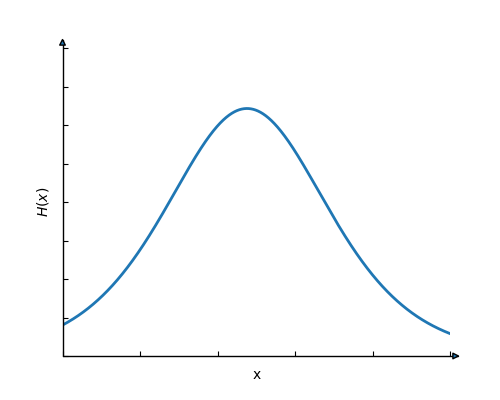
\includegraphics[width=0.40\textwidth]{graphes/CourbeHubbert.png}} 
%    \subfigure{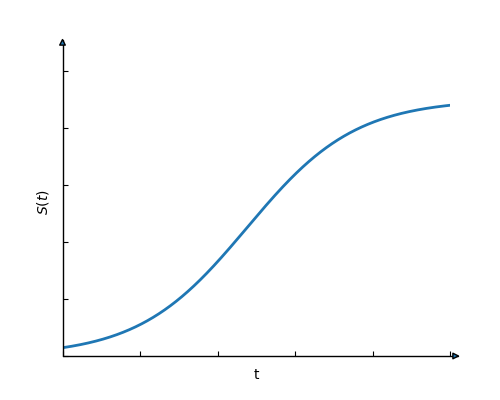
\includegraphics[width=0.40\textwidth]{graphes/Sigmoide.png}} 
%    \caption{Une courbe de Hubbert et sa sigmoïde (son intégrale)}
%    %\label{fig:foobar}
%\end{figure}

$\indent$ Une \textbf{courbe de Hubbert} est une fonction à 4 paramètres : $a$,$b$ et $\tau$, qui définissent sa forme ; et $t$, qui représente le temps. Par la suite, on notera indifféremment $Hubbert_{a,b,\tau}(t)$ ou $H_{a,b,\tau}(t)$.

\begin{equation}\label{linspring}
\begin{gathered}
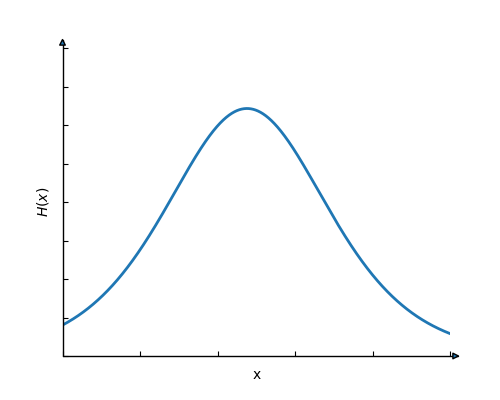
\includegraphics[width=0.40\textwidth]{graphes/CourbeHubbert.png}
\end{gathered}
Hubbert_{a,b,\tau}(t) = \frac{\frac{a b}{\tau} e^{-\frac{t}{\tau}}}{(1+b e^{-\frac{t}{\tau}})^2}
\qquad
\end{equation}
\\
$\indent$ Sa \textbf{sigmoïde} prend quant à elle les 4 paramètres suivants : $S_{max}$,$t_*$ et $\tau$, qui définissent sa forme ; et $t$, qui représente le temps. Par la suite, on notera indifféremment $Sigmoide_{S_{max},t_*,\tau}(t)$, $S_{S_{max},t_*,\tau}(t)$ ou $S(t ; \Theta)$, avec $\Theta = (S_{max},t_*,\tau )$.
\\
\begin{equation}\label{linspring}
\begin{gathered}
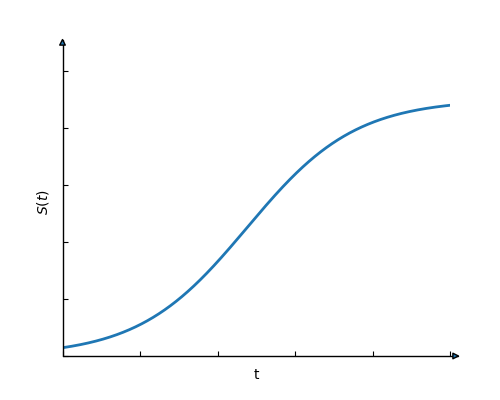
\includegraphics[width=0.40\textwidth]{graphes/Sigmoide.png}
\end{gathered}
Sigmoide_{S_{max},t_*,\tau}(t) = S_{max} \frac{1}{1+ e^{-\frac{(t-t_*)}{\tau}}}
\qquad
\end{equation}

$\indent$ avec $\Delta$ la pente de la sigmoïde au niveau du point d'inflexion $t_*$, et :
\begin{align*}
 S_{max} &= a \indent \indent \text{ le maximum de la sigmoïde}\\
 t_* &= \tau ln(b) \indent \text{le point d'inflexion de la sigmoïde}
\end{align*}

$\indent$ Introduction du modèle mathématique et explication des paramètres
\begin{figure}[h]
	\centering
    \subfigure{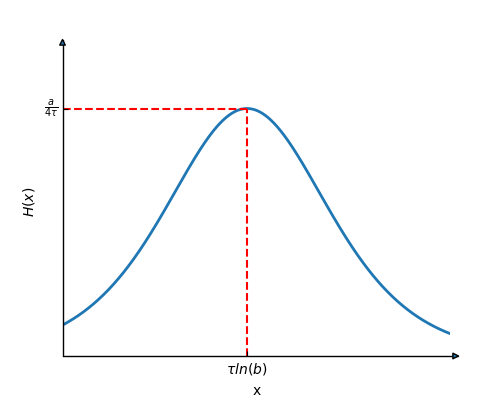
\includegraphics[width=0.6\textwidth]{graphes/Courbe_de_Hubbert_annotée.png}} 
    \subfigure{\includegraphics[width=0.6\textwidth]{graphes/SigmoideAnnotée.png}} 
    \caption{Une courbe de Hubbert et sa sigmoïde (son intégrale)}
    %\label{fig:foobar}
\end{figure}

\newpage






\section{Algorithme d'approximation}
% Explication de l'algorithme et des mathématiques sous jacentes %
$\indent$ Afin d'approximer les paramètres de la sigmoide la plus en adéquation avec nos données, nous allons utiliser la méthode de \textit{descente de gradient}, un algorithme utilisé pour trouver le minimum d'une fonction.



\subsection{Caractérisation}
% Explication détaillées de chaque parties de l'algorithme %
$\indent$ Critères à remplir 
% init dans un intervalle contenant le minimum où S est convexe et lipschitzienne 
% direction de descente
	
$\indent$ Calcul du gradient\\
$\indent$ Mise à jour des paramètres\\
$\indent$ Calcul du critère\\
$\indent$ On recommence jusqu'à atteindre certaines conditions\\



\subsubsection{Critère}
% Explication du critère à optimiser %
$\indent$ Avant toute chose, il nous faut définir un \textit{critère} qui évalue la qualité de notre modèle. Pour cela, nous allons simplement utiliser la distance qui sépare les données de la courbe du modèle. Plus précisément, nous additionnerons pour chaque année le carré de la différence entre l'estimation du modèle et les données réelles.
\begin{equation}\label{eqn:eqCrit}
	C(S(t;\Theta )) = \sum_{k=1}^{N} \delta t | D(t_k) - S(t_k;\Theta ) |^2
\end{equation}
$\indent$ avec :
\begin{center}
	$D(t_k)$ la somme des données de production de l'instant $t_1$ à l'instant $t_k$\\
 	$\delta t$ 
\end{center}



\subsubsection{Gradient}
% Calcule du gradient et de la jacobienne %
$\indent$ Afin de converger vers les paramètres optimaux, l'algorithme de la descente de gradient a besoin d'une direction de descente. Cela passe avant tout par le calcul du gradient de la fonction à minimiser, afin d'avoir une idée précise de l'évolution de cette dernière en fonction de chaque paramètre.\\
$\indent$ A partir de (\ref{eqn:eqCrit}), on obtient :

\begin{equation}\label{linspring}
	\vec{\nabla} C(S(t;\Theta )) = \sum_{k=1}^{N} 2 * \vec{\nabla} S(t_k ;\Theta) * (S(t_k ; \Theta )- D(t_k))
\end{equation}

$\indent$ Il nous faut donc définir $\vec{\nabla} S(\Theta)$ :

$$
\vec{\nabla} S(t;\Theta)= \dfrac{\partial ^2 S}{\partial t \partial \Theta}(t,\Theta ) 
= \left[\begin{array}{c}
\dfrac{\partial S}{\partial t \partial S_{max}}(t,\Theta )\\
\\
\dfrac{\partial f}{\partial t \partial t_*}(t,\Theta ) \\
\\
\dfrac{\partial f}{\partial t \partial \tau}(t,\Theta ) 
\end{array}\right] 
$$

$\indent$ Après calcul, on obtient :

\begin{equation}\label{linspring}
\large \vec{\nabla} S(t;\Theta) = \left[\begin{array}{c}
\frac{1}{1 + e^{-\frac{(t-t_*)}{\tau}}}\\
\\
\frac{- S_{max}}{\tau}*\frac{e^{-\frac{(t-t_*)}{\tau}}}{(1+e^{-\frac{(t-t_*)}{\tau}})^2} \\
\\
\frac{- S_{max}}{\tau ^2}*\frac{e^{-\frac{(t-t_*) * (t-t_*)}{\tau}}}{(1+e^{-\frac{(t-t_*)}{\tau}})^2}
\end{array}\right]
\end{equation}



\subsubsection{Direction de descente}
% Définition de la direction de descente %
\textit{Définition de la direction de descente}



\subsubsection{Figure des isocourbes avec les direction de descentes}
% Affichage de figure, et justification de la nécessité de l'utilisation d'une matrice de mise à l'échelle %
\textit{Affichage de figure, et justification de la nécessité de l'utilisation d'une matrice de mise à l'échelle}



\subsubsection{Matrice de mise à l'échelle}
% Définition de la matrice de mise à l'échelle %
\textit{Définition de la matrice de mise à l'échelle}



\subsubsection{Pseudo code}
% Pseudo Code %
\textit{Pseudo code}



\subsection{Test de contrôle de l'algorithme et des fonctions associées}
% Avant de lancer la l'algorithme sur des données réelles on vérifie que nos fonctions soient justes et que l'algorithme converge pour des données simulées %
\textit{Avant de lancer la l'algorithme sur des données réelles on vérifie que nos fonctions soient justes et que l'algorithme converge pour des données simulées}

\subsubsection{Vérification du gradient par différences finies}
% Test rapide du gradient par la méthode des différences finies %
\textit{Test rapide du gradient par la méthode des différences finies}

\subsubsection{Test de convergence avec données bruitées et non bruitées, en commençant plus ou moins loin de la solution}
% Test rapide de convergence l'algorithme sur des données générées, il y aura 4 tests comme précisé dans le titre se la sous-section %
\textit{Test rapide de convergence l'algorithme sur des données générées, il y aura 4 tests comme précisé dans le titre se la sous-section}

\subsection{Performance \textit{-optionnel}}
% Test des performances de l'algorithme %
\textit{Test des performances de l'algorithme}

\subsubsection{Temps de convergence selon diffèrent paramètre}
% Différents tests sur la vitesse de convergence sur par exemple :  le niveau de bruit, la distance de départ par rapport à la solution, facteur de rebroussement, etc %
\textit{Différents tests sur la vitesse de convergence sur par exemple : le niveau de bruit, la distance entre le point de départ et la solution, le facteur de rebroussement, etc }

\section{Données réels}
% Après l'introduction de l'algorithme, introduction de l'algorithme aux données réelles et évaluation des ces performances %
\textit{Après l'introduction de l'algorithme, introduction de l'algorithme aux données réelles et évaluation des ces performances}

\subsection{Vérification de la pertinence du modèle}
% Application de l'algorithme sur un jeu de données pertinentes %
\textit{Application de l'algorithme sur un jeu de données pertinentes}

\subsubsection{Vérification de la pertinence du modèle sur plusieurs set de donnés \textit{-optionnel}}
% Généralisation du test de pertinence %
\textit{Généralisation du test de pertinence}

\subsubsection{Vérification de la pertinence sur la somme de la production mondiale \textit{-optionnel}}
% Test de la pertinence du modèle sur une vue globale %
\textit{Test de la pertinence du modèle sur une vue globale}

\subsubsection{Explication des lacunes du modèle}
% Après avoir mit en exergue les lacunes sur quelques jeux de données, tentatives de caractérisations des hypothèses de validité du modèle %
\textit{Après avoir mit en exergue les lacunes sur quelques jeux de données, tentatives de caractérisations des hypothèses de validité du modèle}

\subsection{Pic de production \textit{-optionnel}}
% Vérification de la performance de l'algorithme pour trouver les pics de production %
\textit{Vérification de la performance de l'algorithme pour trouver les pics de production}

\subsubsection{Vérification de la performance de l'algorithme pour trouver les pics de production a posteriori}
% La détermination du pics étant simple a posteriori, on peut calculer de la performance de l'algorithme à trouver le pic de production a posteriori %
\textit{La détermination du pics étant simple a posteriori, on peut calculer de la performance de l'algorithme à trouver le pic de production a posteriori}

\subsubsection{Performance de l'algorithme pour trouver les pics de production sur les données qui peuvent être modélisées par une sigmoïde}
% En prenant des sets de données qui peuvent être convenablement modélisé par une sigmoïde, on peut cherche à quel point le modèle est prédictif. Pour cela on calcul la précision avec laquelle l'algorithme prédit le pic de production en se limitant aux premières données jusqu'à un temps $t$ %
\textit{En prenant des sets de données qui peuvent être convenablement modélisé par une sigmoïde, on peut cherche à quel point le modèle est prédictif. Pour cela on calcul la précision avec laquelle l'algorithme prédit le pic de production en se limitant aux premières données jusqu'à un temps $t$}

\subsection{Amélioration de modèle}
% Avec un algorithme flexible, on peut essayer d'améliorer la modélisation %
\textit{Avec un algorithme flexible, on peut essayer d'améliorer la modélisation}

\subsubsection{Deux sigmoïdes}
% Si il y a deux pics, est-ce que deux sigmoïdes additionnées est un bonne modélisation? %
\textit{Si il y a deux pics, est-ce que deux sigmoïdes additionnées est un bonne modélisation?}

\subsubsection{n sigmoïdes}
% Si il y a n pics, est-ce que n sigmoïdes additionnées est un bonne modélisation? %
\textit{Si il y a n pics, est-ce que n sigmoïdes additionnées est un bonne modélisation?}

\section{Conclusion}
\end{document}
